\section{Experiments and Results}
\subsection{Measured S-Parameters}
Figs.~\ref{fig:s11_plot} and~\ref{fig:s21_plot} present the simulated and measured $S_{11}$ and $S_{21}$ parameters, respectively, over the DC--5\,GHz range. A resonance outside the band of interest was identified in the measured response. This feature was not predicted by the original simulation model and is attributed to parasitic effects of the PCB layout and component packaging that were not fully captured in the initial model.

The measured center frequency is 2.11\,GHz, corresponding to a 90\,MHz shift from the design target of 2.2\,GHz. This shift is attributed to the series equivalent inductance (ESL) of the stabilization resistors, which was not accounted for in the original model. Incorporating an ESL of 0.5\,nH per resistor, a value consistent with published data for 0603-package thin-film resistors \cite{VishayTN}, brings the simulated center frequency into agreement with the measurement. The overall small-signal behavior closely matches the design objectives.

\begin{figure*}[t]
    \centering
    \begin{minipage}{0.48\textwidth}
        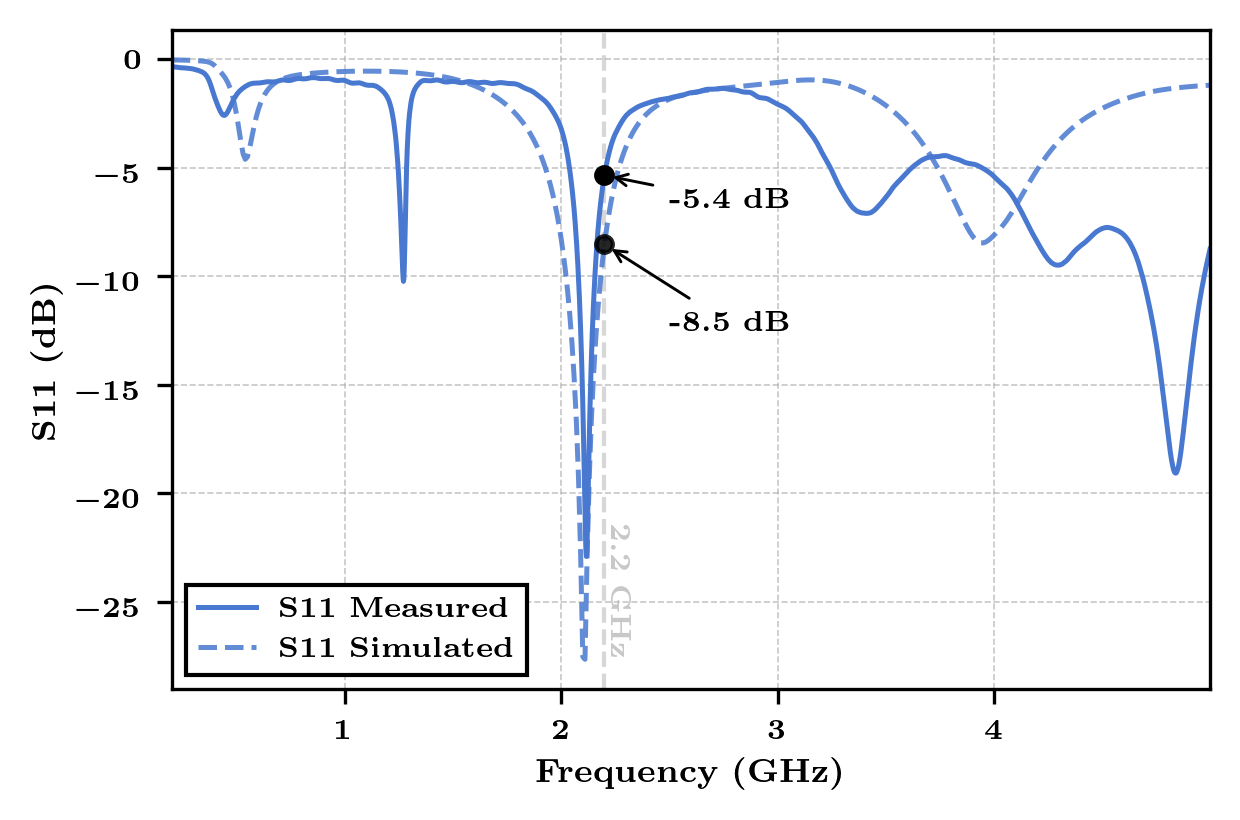
\includegraphics[width=\linewidth]{imgs/s11_plot.png}
        \caption{Comparison of the simulated (dashed line) and measured (solid line) $S_{11}$ of the fabricated power amplifier.}
        \label{fig:s11_plot}
    \end{minipage}
    \hfill
    \begin{minipage}{0.48\textwidth}
        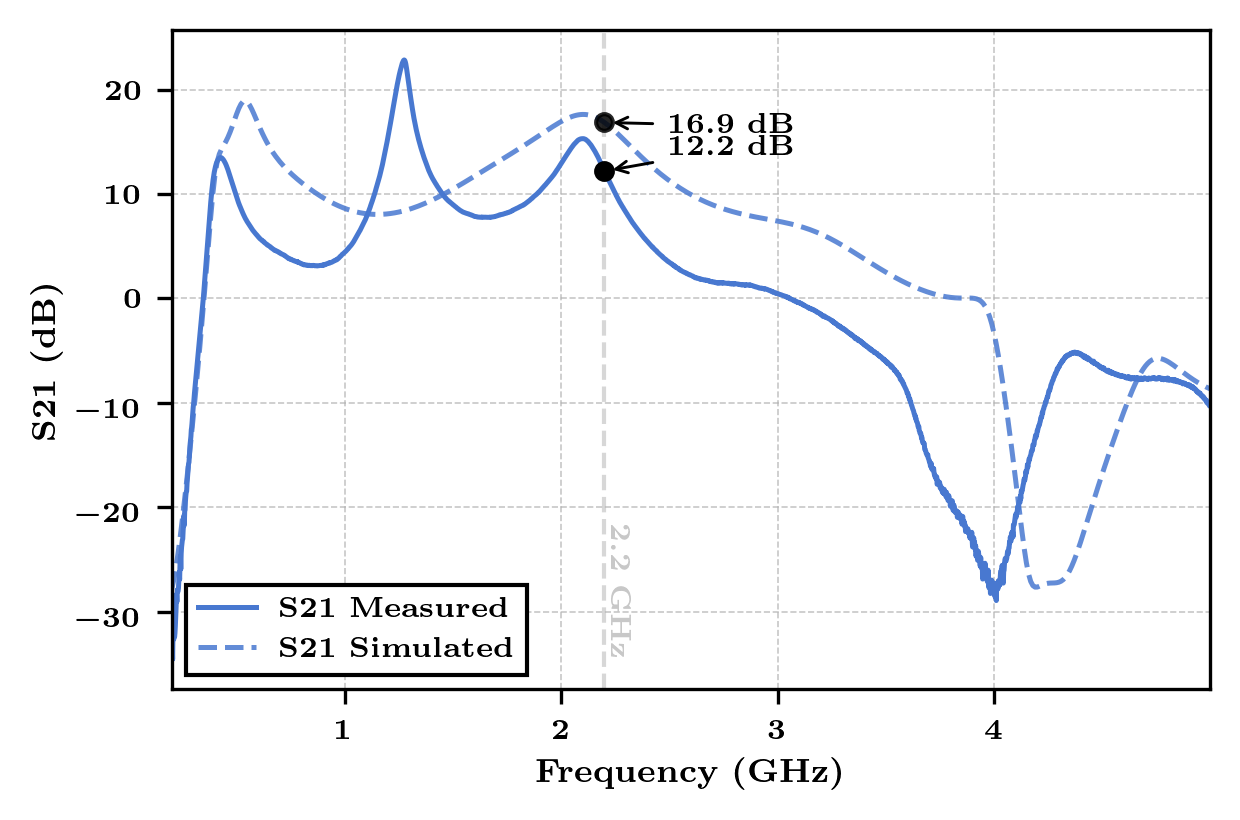
\includegraphics[width=\linewidth]{imgs/s21_plot.png}
        \caption{Comparison of the simulated (dashed line) and measured (solid line) $S_{21}$ of the fabricated power amplifier.}
        \label{fig:s21_plot}
    \end{minipage}
\end{figure*}

% =========================================================================== %
\subsection{P1dB Extraction}
The 1\,dB gain compression point (P1dB) is a key figure of merit for power amplifiers, defined as the input power level at which the output power deviates by 1\,dB from the extrapolated small-signal linear response. It marks the boundary of the amplifier's linear operating region \cite[pp.~512--513]{Pozar2012}.

Fig.~\ref{fig:p1db_img} shows the measured output power as a function of input power for the complete test chain (driver amplifier and PA under test). Because the driver amplifier itself enters compression within the measurement range, the P1dB of the system under test cannot be read directly from the measured output power curve. Instead, the cascade compression expression~\eqref{eq_p1db} was applied, which refers the compression of each stage to the system input and combines their contributions inversely weighted by the gain of the preceding stages~\cite{Dong2021}. The PA P1dB was extracted by solving this expression using the known gain and compression values of the driver stage, yielding a P1dB of 30.3\,dBm at an operating frequency of 2.2\,GHz.

\begin{equation}
    \scalebox{0.85}{$\displaystyle 
        \frac{1}{P_{1dB_{sys}}} = \frac{1}{G_2\cdots G_N P_{1dB_1}} + \frac{1}{G_3\cdots G_N P_{1dB_2}} + \cdots + \frac{1}{P_{1dB_N}}$
    }
    \label{eq_p1db}
\end{equation}

\begin{figure}[t!]
    \centering
    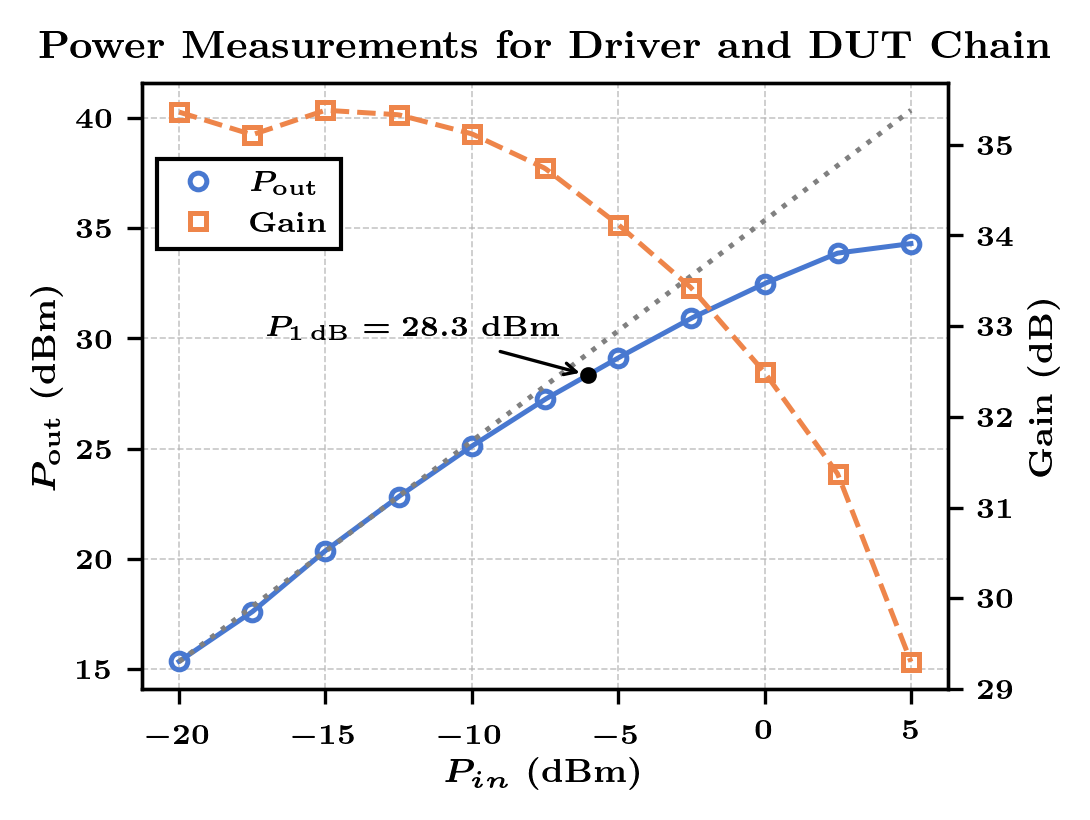
\includegraphics[width=0.48\textwidth]{imgs/p1db_plot.png}
    \caption{Measured output power (blue) and gain (orange) as a function of input power for the driver-DUT chain. The dotted gray line represents the ideal linear transfer characteristic obtained from the small-signal gain extrapolation.}
    \label{fig:p1db_img}
\end{figure}

% =========================================================================== %
\subsection{Gain, Drain efficiency and Bandwidth}
\subsubsection{Gain}
The small-signal gain of the amplifier was extracted from the power measurement chain. The input and output power at the PA terminals were computed as:

\begin{align}
    P_{in,PA}  &= P_{in,sys} + G_{driver} \label{eq_pin} \\
    P_{out,PA} &= P_{out,sys} + |A_{att}| \label{eq_pout}
\end{align}

where $P_{in,sys}$ is the system input power, $G_{driver}$ is the gain of the driver stage, $P_{out,sys}$ is the measured system output power, and $|A_{att}|$ is the total attenuation of the attenuator chain, with all quantities in dBm and dB respectively. The gain was then calculated as:

\begin{equation}
    G = P_{out,PA} - P_{in,PA}
    \label{eq_gain}
\end{equation}

A small-signal gain of 13.26\,dB was obtained.

% =========================================================================== %
\subsubsection{Drain Efficiency}
Drain efficiency ($\eta_D$) was evaluated at the measurement point closest to the 1\,dB compression point, corresponding to an output power of 30.92\,dBm, and computed as:

\begin{equation}
    \eta_D = \frac{P_{out,PA}}{P_{DC}} \times 100\%
    \label{eq_eta}
\end{equation}

where $P_{out,PA}$ is the output power delivered by the amplifier and $P_{DC}$
is the DC power consumed. A drain efficiency of 32.94\% was obtained. The power-added efficiency at the same operating point, computed as

\begin{equation}
    \text{PAE} = \frac{P_{out,PA} - P_{in,PA}}{P_{DC}} \times 100\%,
    \label{eq_pae}
\end{equation}

was 30.51\%.

\subsubsection{Bandwidth}
The operating bandwidth was determined from the measured $S_{11}$ response. The two frequency points at which $S_{11}$ crosses the $-10$\,dB threshold within the region of interest were identified, and the bandwidth was defined as their difference, obtaining a 70\,MHz value.

% =========================================================================== %
\subsection{Measured Harmonic Distortion}
The second and third harmonics were measured at $P_{in}=20\,\text{dBm}$, approximately at the P1dB operating point, representing the worst-case nonlinear condition during normal amplifier operation. The second harmonic rejection was 26.74 dBc and the third harmonic rejection was 42.21 dBc. These values represent the minimum expected performance in linear operation below P1dB. The measured harmonic content differs from the simulation model, which is attributed to a frequency shift in the output filter's rejection band. This can be observed in the amplifier's forward transmission response (S21), where the output filter stopband appears shifted toward lower frequencies.


% =========================================================================== %
\subsection{Measured OIP3}
The output-referred third-order intercept point (OIP3) is another parameter that characterizes the nonlinear behavior of the amplifier. It is a figure of merit that indicates the output power at which the third-order intermodulation products (IM3) become comparable to the fundamental signal. It is an important value as the IM3s are typically encountered in the operating band. The OIP3 is a theoretical point defined as the intersection of the extrapolation of the output power transfer curve with respect to the input power, with a unity slope on a log-log scale, and the extrapolation of the IM3 response as a function of the input power, where the slope is 3 dB/dB for the same scale ~\cite[pp.~515--517]{Pozar2012}.

The OIP3 was determined for the driver and power amplifier chain. Fig.~\ref{fig:oip3} shows the OIP3 of the chain for a wide range of frequencies. As with the P1dB, the nonlinearity of the driver amplifier affects the chain OIP3. For this reason, the OIP3 value for the DUT was obtained from equation ~\eqref{eq_oip3}.

\begin{equation}
    \scalebox{0.85}{$\displaystyle 
        OIP3_{sys} = \left(\frac{1}{OIP3_{N-1} \cdot G_N} + \frac{1}{OIP3_N}\right)^{-1}$
    }
    \label{eq_oip3}
\end{equation}

An OIP3 of $39.83\,\text{dBm}$ was obtained. This value is consistent with the expected experimental relationship between the P1dB and the OIP3, where the OIP3 is usually 10 to 15 dB larger than the P1dB~\cite[p.~516]{Pozar2012}.

\begin{figure}[b]
    \centering
    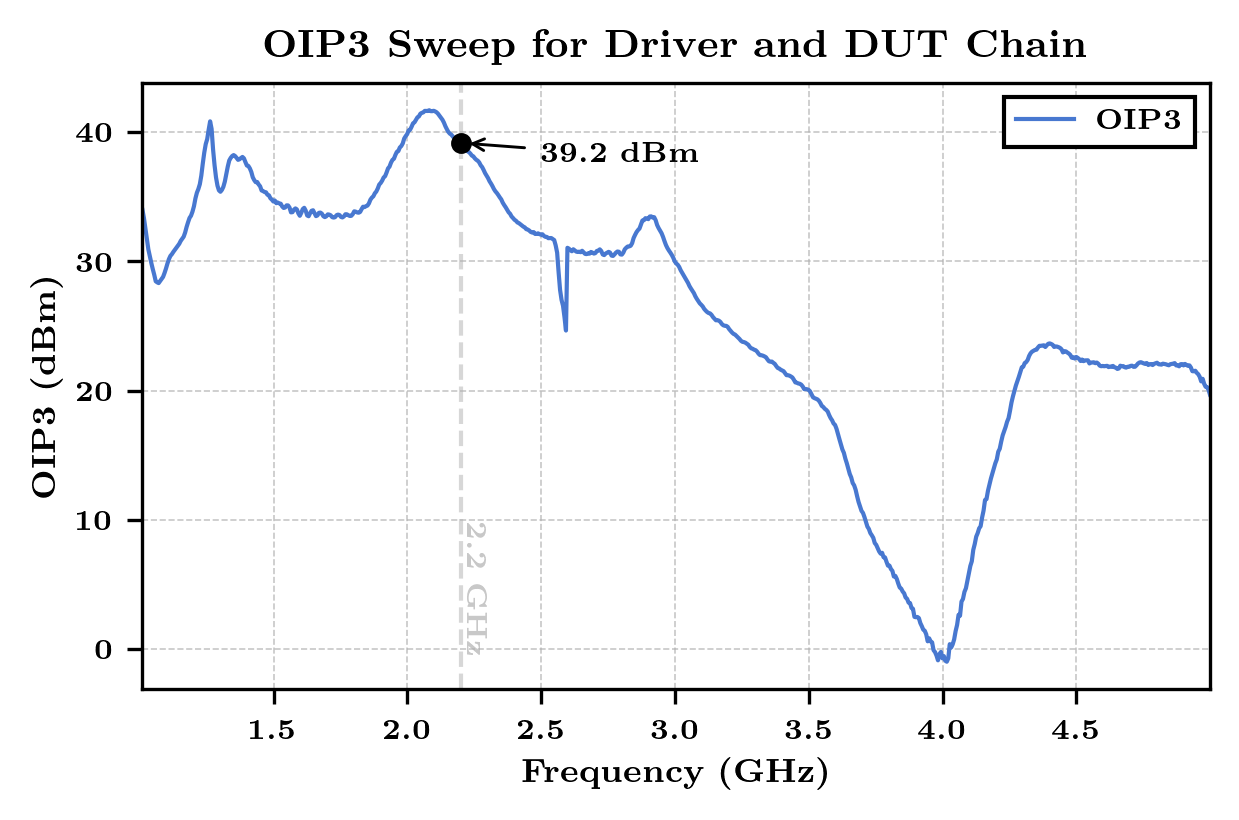
\includegraphics[width=1\linewidth]{imgs/oip3_plot.png}
    \caption{Frequency sweep of the measured output third-order intercept point (OIP3) for the driver–DUT chain.}
    \label{fig:oip3}
\end{figure}


% =========================================================================== %
\subsection{Summary of Results}
Table~\ref{tab:pa_results} summarizes the key measured performance parameters of the fabricated amplifier, providing a consolidated overview of the characterization results presented throughout this section.

\begin{table}[ht]
    \caption{RF Power Amplifier Measured Performance Summary}
    \label{tab:pa_results}
    \centering
    \renewcommand{\arraystretch}{1.15}
        \begin{tabular}{lc}
        \hline\hline
        \textbf{Parameter}                         & \textbf{Value}                 \\
        \hline
        Center Frequency                           & 2.11\,GHz                      \\
        Bandwidth (BW)                             & 70\,MHz                        \\
        1\,dB Compression Point ($P_{1\text{dB}}$) & 30.30\,dBm                     \\
        Third-Order Intercept ($\text{OIP}_3$)     & 39.83\,dBm                     \\
        Small-Signal Gain                          & 13.26\,dB                      \\
        Drain Efficiency                           & 32.94\% @ $P_{out}=30.92$\,dBm \\
        PAE                                        & 30.51\% @ $P_{out}=30.92$\,dBm \\
        VSWR                                       & $<$1.92:1                      \\
        \hline\hline
        \end{tabular}
\end{table}